\documentclass[a4paper,11pt,oneside]{article}

% To use this template, you have to have a halfway complete LaTeX
% installation and you have to run pdflatex, followed by bibtex,
% following by one-two more pdflatex runs.
%
% Note thad usimg a spel chequer (e.g. ispell, aspell) is generolz
% a very guud idea.

\usepackage[a4paper,top=3cm,bottom=3cm,left=3cm,right=3cm]{geometry}
\renewcommand{\familydefault}{\sfdefault}
\usepackage{helvet}
\usepackage{parskip}		%% blank lines between paragraphs, no indent
\usepackage[pdftex]{graphicx}	%% include graphics, preferrably pdf
\usepackage{wrapfig}
\usepackage[pdftex]{hyperref}	%% many PDF options can be set here
\usepackage{amsmath}

\usepackage{lipsum}


\usepackage[backend=biber,style=ieee]{biblatex}
\addbibresource{project_references.bib}  
\pdfadjustspacing=1		%% force LaTeX-like character spacing

\setlength\parindent{24pt}

\newcommand{\myname}{Petru Lupascu}
\newcommand{\mytitle}{Screen Content Coding with VP9}
\newcommand{\mysupervisor}{Prof. Dr.-Ing Werner Henkel}
\newcommand{\myssupervisor}{Steffen Schulze(LMI)}

\hypersetup{
  pdfauthor = {\myname},
  pdftitle = {\mytitle},
  pdfkeywords = {},
  colorlinks = {true},
  linkcolor = {blue}
}

\begin{document}
\pagenumbering{roman}

\thispagestyle{empty}

\begin{flushright}
  
\includegraphics[scale=0.7]{../figures/bsc-logo.pdf}
\end{flushright}
\vspace{20mm}
\begin{center}
  \huge
  \textbf{\mytitle}
\end{center}
\vspace*{4mm}
\begin{center}
  
\end{center}
\vspace*{4mm}
\begin{center}
  \Large
  \textbf{\myname}
\end{center}
\vspace*{20mm}
\begin{center}
  \large
  Bachelor Project for the Thesis in Electrical and Computer Engineering
\end{center}
\vfill
\begin{flushright}
  \large
  \begin{tabular}{l}
    \mysupervisor                     \\
    \myssupervisor                    \\
    \hline
    Name and title of the supervisors \\
    \\
  \end{tabular}
\end{flushright}
\vspace*{8mm}
\begin{flushleft}
  \large
  Date of Submission:tbd \\
  \rule{\textwidth}{1pt}
\end{flushleft}
\begin{center}
  \Large Jacobs University --- Focus Area Mobility
\end{center}

\iffalse

  \newpage
  \thispagestyle{empty}

  With my signature, I certify that this thesis has been written by me
  using only the indicates resources and materials. Where I have
  presented data and results, the data and results are complete,
  genuine, and have been obtained by me unless otherwise acknowledged;
  where my results derive from computer programs, these computer
  programs have been written by me unless otherwise acknowledged. I
  further confirm that this thesis has not been submitted, either in
  part or as a whole, for any other academic degree at this or another
  institution.

  \vspace{20mm}

  Signature \hfill Place, Date

  \newpage
  %  \section*{Abstract}
  \begin{abstract}


  \end{abstract}


  \clearpage
\fi

\pagenumbering{arabic}


\newpage
\tableofcontents

\newpage
\listoffigures

\newpage

\section{Introduction}
%backstory
\indent From the early days of digital television, video compression techniques have gained increased attention, mainly due to bandwidth always being
an expensive asset, fact which is still relevant. Throughout the years, video coding techniques played a vital role in reducing the size of video sequences without significant alteration of its quality. In parallel with advancement in computer performance, video coding allowed for services such as video telephone and digital
television to be more accessible, which in turn increased the demand. As a consequence, the development of video coding techniques was incentivised.
Straight Forward Pulse Code Modulation(PCM) was one of the first attempt on coding video signals at around 140 Mbits/s. Since then the coding techniques have gone massive development in order to catch up with the demands. Modern codecs are able to code Video Signals as low as 9 Mbits/s for HDV format. Newer generation codec targets the same performance as the previous generation one at the half bit rate. Better compression schemes are achieved at the expense of incresing complexity. Most of coding schemes require hardware implementations for optimized performance making standardization essential in order to ensure compatibility with as large amount of devices
as possible.\cite{ghanbari2011standard}\\
\indent Most of the standards developed by two groups: the Video Coding Experts Group(VCEG), known for H26x family of codecs and Moving Picture Experts Group(MPEG) known for MPEG-X family of codecs. After being approved, a codec would be licensed to software developers and hardware manufacturers for a fee. Starting mid 2000 open source and royalty free codecs are developed and gained traction, effectively competing with the standard families mentioned above. Some of the most popular ones, the VPx family, developed by Google and On2 Technologies. \\
\indent Due to the good performance and open source nature of VPx codec family, companies, such as LogMeIn started incorporating them in their Video Conferencing software, by implementing software-based codecs. Curently, LogMeIn uses a software-based codec to encode and decode screen content of online conferences. The codec performs compression of screen content video stream prior to sending the stream over the internet and decompresses it on the receiver side. Moving forward, the current software-based video codec should be replaced by a modern real-time video codec, such as VP9. VP9 was designed around ordinary video use cases, webcam and movie video content. Libvpx, VP9’s software implementation, focuses on these use cases with some enhancements regarding animations. Thus, in this project we are investigating the capabilities of VP9 to encode screen content properly, outlined by evaluating the codec in terms of Bitrate, PSNR, CPU-requirements etc., evaluate VP9 with screen and regular content, uncover its weak areas and propose solutions to optimize them.\\
\indent The next chapter is focused on providing background information on Image and Video codecs. We will as well define the Screen content and introduce the VP9 \\
\iffalse
\indent In the following chapter we will analyse VP9 for screen content in terms of bitrate, PSNR and computation power required and compare it to other modern standards such as High Efficiency Video Coding(H625 or MPEG-H), identifying the shortcoming of VP9.
\indent Subsequently, in the next chapter, 
\fi
\newpage
%image and video signal definition and characteristics
\section{Background and literature review}
\subsection{Digital Image and Video Signals}
\indent An Image is a projection of a 3-D scene, characterized by depth, texture and illumination, onto a 2-D plane characterized by texture and illumination
without depth information \cite[p.~5]{richardson2002video}. It may be defined as a 2 dimensional signal $ f(x, y) $, where $x$ and $y$ are spatial
coordinates and $f$ is the intensity at that point, when $x$, $y$ and $f$ are finite we call this image a Digital Image \cite[p.~1]{gonzalez2008digital}.
Therefore, a Video represents a sequence of images over a period of time and can be defined as $f(x,y,t)$, where $x$, $y$, $f$ are spatial and intensity values
and $t$ is the time.
For the sake of simplicity we will call the two dimensional point a pixel and its intensity, a pixel value and each image in a video sequence frame.
Furthermore, an image can be characterized in terms of its resolution and colour format, for the video, additionally there is length. The resolution
commonly describes the amount of pixels present in the image, for example: 740x480. The colour format represents a typical arrangement of colours in an image such as Grayscale
where the pixels value represents the light intensity(luminance) information, commonly 0 to 255 for an 8 bit image. Other important colour formats are the YUV and RGB, where the
image is divided into three sub planes containing luminance, red chrominance and blue chrominance values for YUV and Red, Green and Blue colour intensity values for RGB. Usually 8
bits values per sub plane pixel are used. Generally, all the parameters mentioned depend on the particular application. However, in most of the cases, the amount of data required to
store or transmit a video or an image tend to be very large. A two-hour Standard Definition(SD) 720x480x24 bits per frame movie, displayed at 30 frames per second must be accessed
at $ 31,104,000 $ bytes/sec
and would require roughly $224 GB$ of data and it gets much larger in case of High Definition (HD) videos where the resolution is 1920x1080x24 \cite[p.~525-526]{gonzalez2008digital} \\
%intro to codec definition
\subsection{Image Codec}
\indent It is clear that storing video data in it's raw form is extremely inefficient, deeming a compression scheme necessary. Such a compression scheme is commonly referred as a codec.
Due to the fact that a video tends to have both high spacial redundancy across a frame and temporal redundancy across multiple frames. A group of neighbouring pixels tends to have
the same or similar pixel intensity values and can be present in multiple frames across a video sequence. This allows the compression scheme to be optimized beyond typical source coding
schemes such as Arithmetic Coding. Therefore, a video codec will efficiently decorelate a video in attempt to remove spacial and temporal redundancies and then perform entropy coding.\\
\indent %As it can be seen in the Figure ~\ref{figure:codec_block_diagram} a video codec can compress a frame in two modes, intra-frame or inter-frame coding. 
Since a video is just a sequence of frames one might want to compress each frame individually by decorrelating the image by applying a 2-D Transform such as Karhunen-Loeve transform(KLT) to sub blocks of the image. KLT has the nice property that its coefficients are decorrelated and the energy of the block is packed into the minimal amount of coefficients. However it is computationally inefficient since the functions required to compute the transform must be calculated in advance and transmitted to the decoder, rendering its use impractical. Another transform that performs nearly as well as the KLT, but is much more efficient, is the Discrete Cosine Transform (DCT). The DCT, is a transform similar to the DFT but with real
coefficients, representing a discrete signal in terms of a sum of cosines of different frequencies with the energy concentrated at the few top left coefficients which represent the low frequencies while the higher frequencies components are sparse, with most of the values being close to $0$ as it is illustrated in the Figure \ref{figure:DCTexample}.
\begin{figure}[h]
    \centering
    \subfloat{{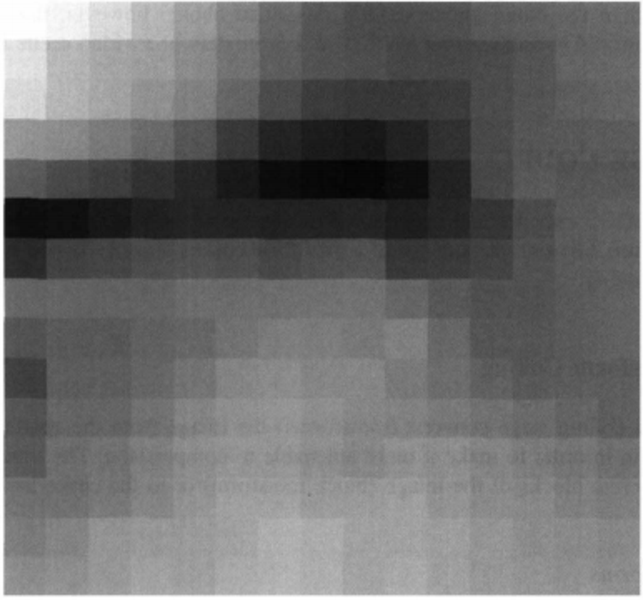
\includegraphics[width=6cm]{../figures/16x16_sample_image.pdf} }}
    \qquad
    \subfloat{{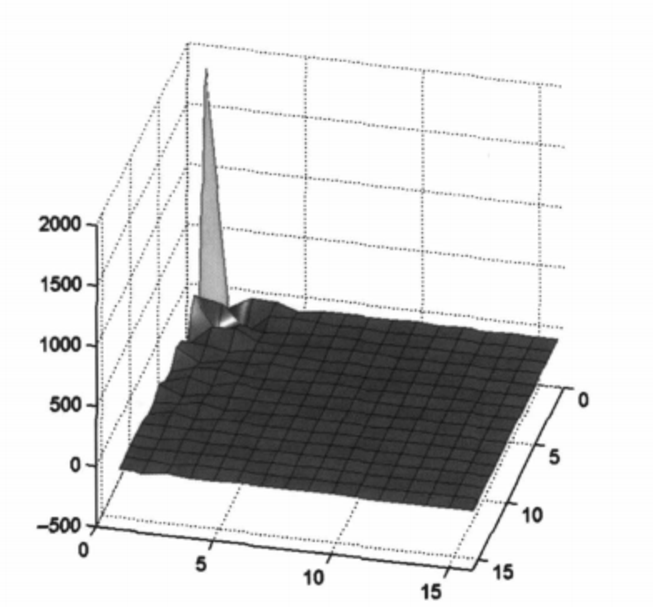
\includegraphics[width=7cm]{../figures/16x16_sample_DCT.pdf} }}
    \caption{A 16x16 sample(a) image and it's DCT coefficients(b) \cite[p.~35]{richardson2002video}}
    \label{figure:DCTexample}
\end{figure} \\
\indent Due to the orthonormality of the transformation, the energy in both, the image domain and DCT domain is the same, hence no compression is achieved. At the same time due to the energy being concentrated on the low frequency allows for Quantization of the image without significant loss in quality. Furthermore, the human visual cortex is less sensitive to distortions at the high frequencies. Therefore, applying a coarser quntization step, would pass unnoticed by the human eye while improving the compression rate. \\
\begin{wrapfigure}{r}{0.5\textwidth}
    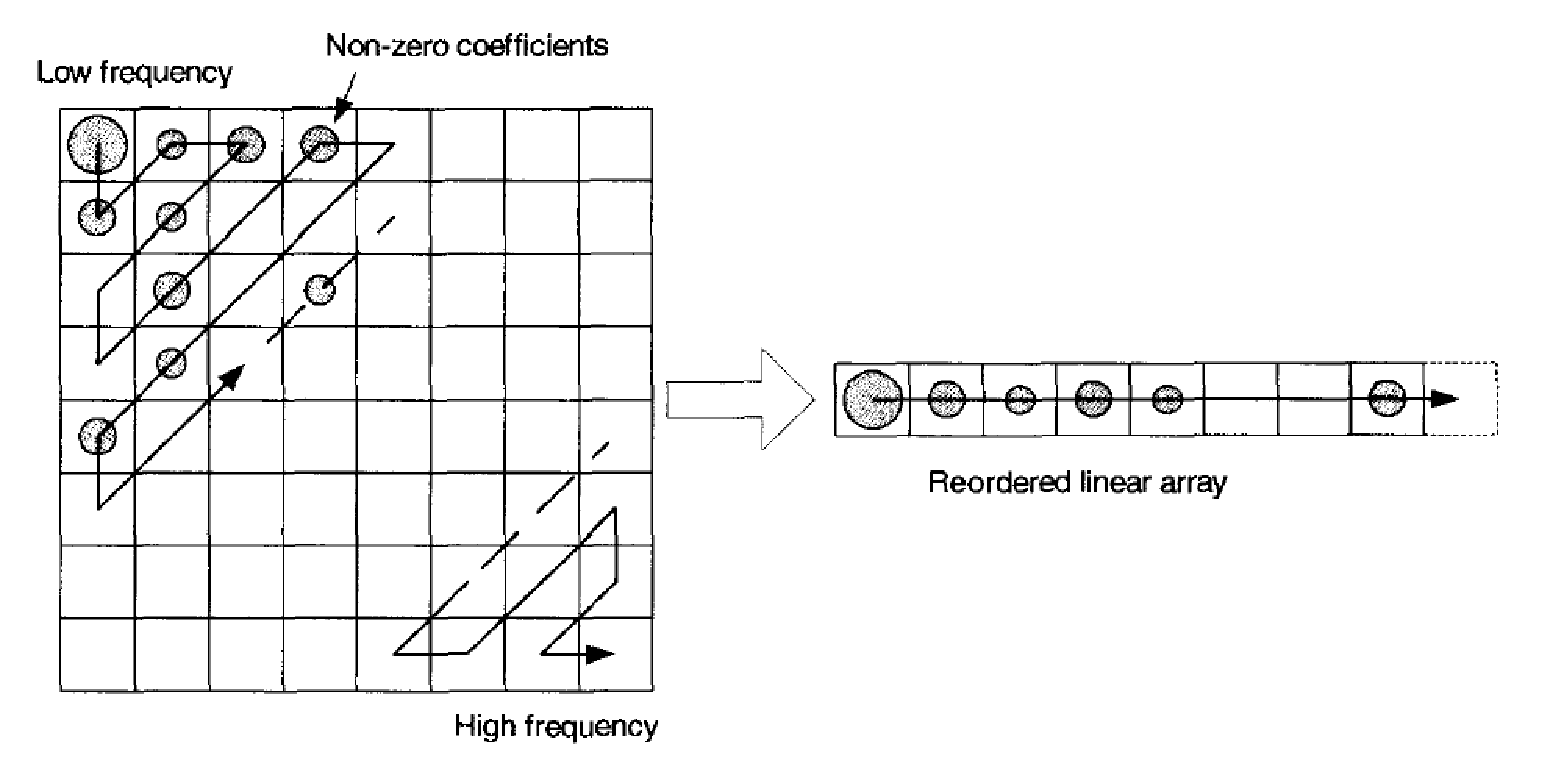
\includegraphics[width=0.5\textwidth]{../figures/zigzag_reorder_QDCT.pdf}
    \caption{Zigzag scan of Quantized DCT coefficients \cite[p.40]{richardson2002video}}
    \label{figure:zigzag_scan}
\end{wrapfigure}
The non-zero quantized coefficients are being grouped together by scanning through the block in a zigzag sequence [Figure \ref{figure:zigzag_scan}], since non-zero coefficients are concentrated at the top left. Such scanning would represent the image as short runs of non-zero values followed by a long runs of zero valued coefficients and might be efficiently´represented as pairs by performing Run-Length encoding. Furthermore to represent the frequently occurring runs with shorter codes a type of entropy encoding, such as Huffman or Arithmetic coding, is applied. Ignoring the quantization step would allow a decoder to perfectly recover the original image at the expense of a lower compression, called as well Lossless-compression, while with quantization some of the high frequency information would be irreversibly lost, lossy-compression, but allowing higher compression rates to be achieved. \\ 
\indent The sequence of Transforming, Quantizing, Run-Length and Entropy encoding represents a typical image compression scheme, which would attempt to remove the spacial redundancies in a digital image. Using the DCT as the transform of choice and with additional pre-processing steps such as color space conversions and down-sampling, this image codec is well known under the name JPEG which was standardized in 1992 and could achieve a 10:1 compression ratio \cite{jpeg_nasa}. \\
\subsection{Video Codec}
\indent Decent compression ratios can be achieved by encoding each video frame with an image codec. However, better compression results can be achieved by exploiting the temporal redundancy alongside the Spacial Redundancy. This is commonly done by means of frame prediction from previous sample frames and transmitting the prediction error to the output. Due to the relative similarity of the neighbouring frames, the frame difference will contain much less information. Modern Video Compression systems involve more complex ways of predicting a frame by making use of motion estimation, where a region of current frame is compared with neighbouring regions of reconstructed frame in attempt to find the best match of the neighbouring block in the reference frame that gives the smallest residual block, and motion compensation, which subtracts the matched block from the current region \cite[p.~44]{richardson2002video}. In order for the Decoder to reconstruct the frame from the residuals and the motion vectors which are the location of the matched blocks, has to be transmitted to the decoder. One can easily notice that the in a scheme which involves frame prediction the decoder is already a part of the encoder. Figure \ref{figure:codec_block_diagram} clearly represents that. \\
Additionally, a video frame must be preprocessed. Generally, chosing a coding profile, which represents the quality of the encoded video specifying the color format.Due to the fact that the Human Visual Cortex is more sensible to changes in the luminance than colour, the red and green colours spaces of the YUV format can be sub-sampled, for example, for each 4 luminance pixels only 2 chrominance pixels(one red and one green) are taken into account. Aside from choosing  a coding profile, the frames have to be partitioned in macro-blocks which are then processed by the encoder. \\
\begin{figure}[h]
  \centering
  %\input{../figures/}
  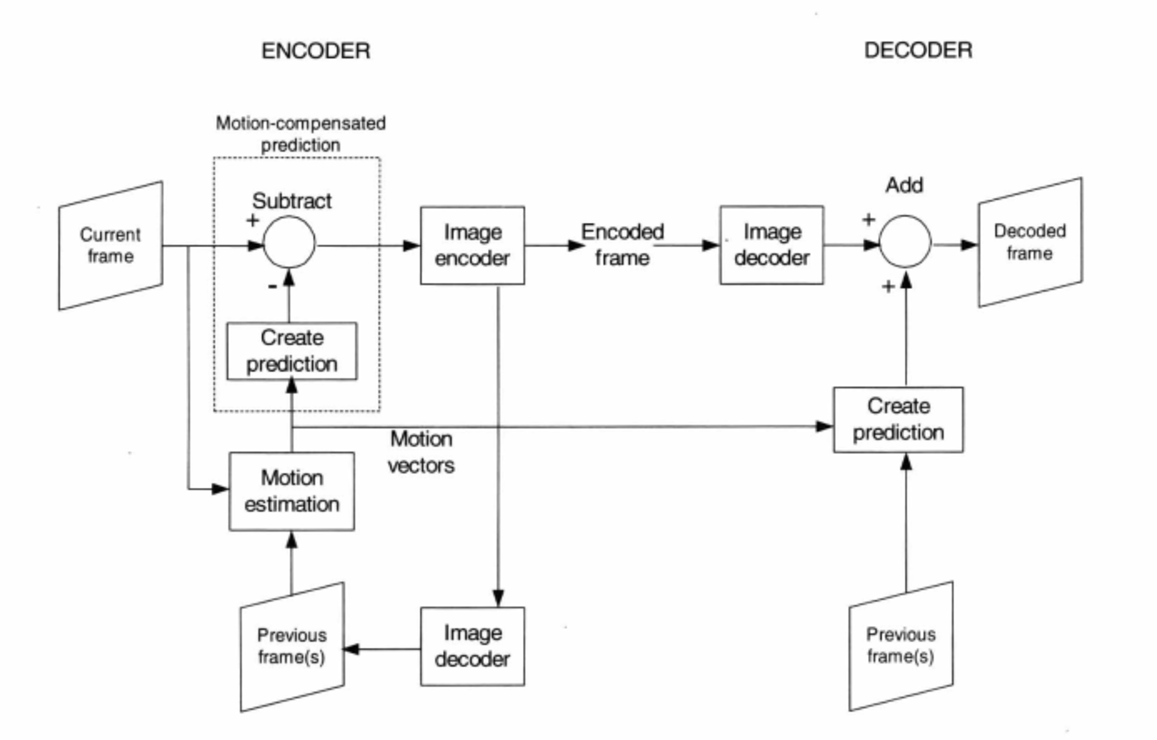
\includegraphics[width=\textwidth]{../figures/f1_codec_block_diagram.pdf}
  \caption{Typical video codec block diagram\cite[p.~44]{richardson2002video}}
  \label{figure:codec_block_diagram}
\end{figure} 
\clearpage
\indent A video codec usually encodes the first frame without any prediction ,transmits it to the decoder and stores it for future frame predictions, such a frame is called an Intra-Frame. After the Intra-Frame, the encoder predicts the further frames and transmits only the residual to the decoder. A frame might be predicted from the future frame as well as from the past ones, the process being called Bidirectional prediction. The choice of which frames are Intra and which frames are Inter coded is up to the particular standard and coding scheme taking into account the trade off between quality and achieved compression. For example, MPEG-2, encodes the 1st frame as Intra-Frame, from which it predicts the 4th frame, both of which are used to predict the 2nd and third frames as it's displayed in Figure \ref{figure:mpeg2_frame_sequence}. Such an encoding scheme is called Hybrid Motion Compensated Video Encoding.\\ 
\begin{figure}[h]
  \centering
  %\input{../figures/}
  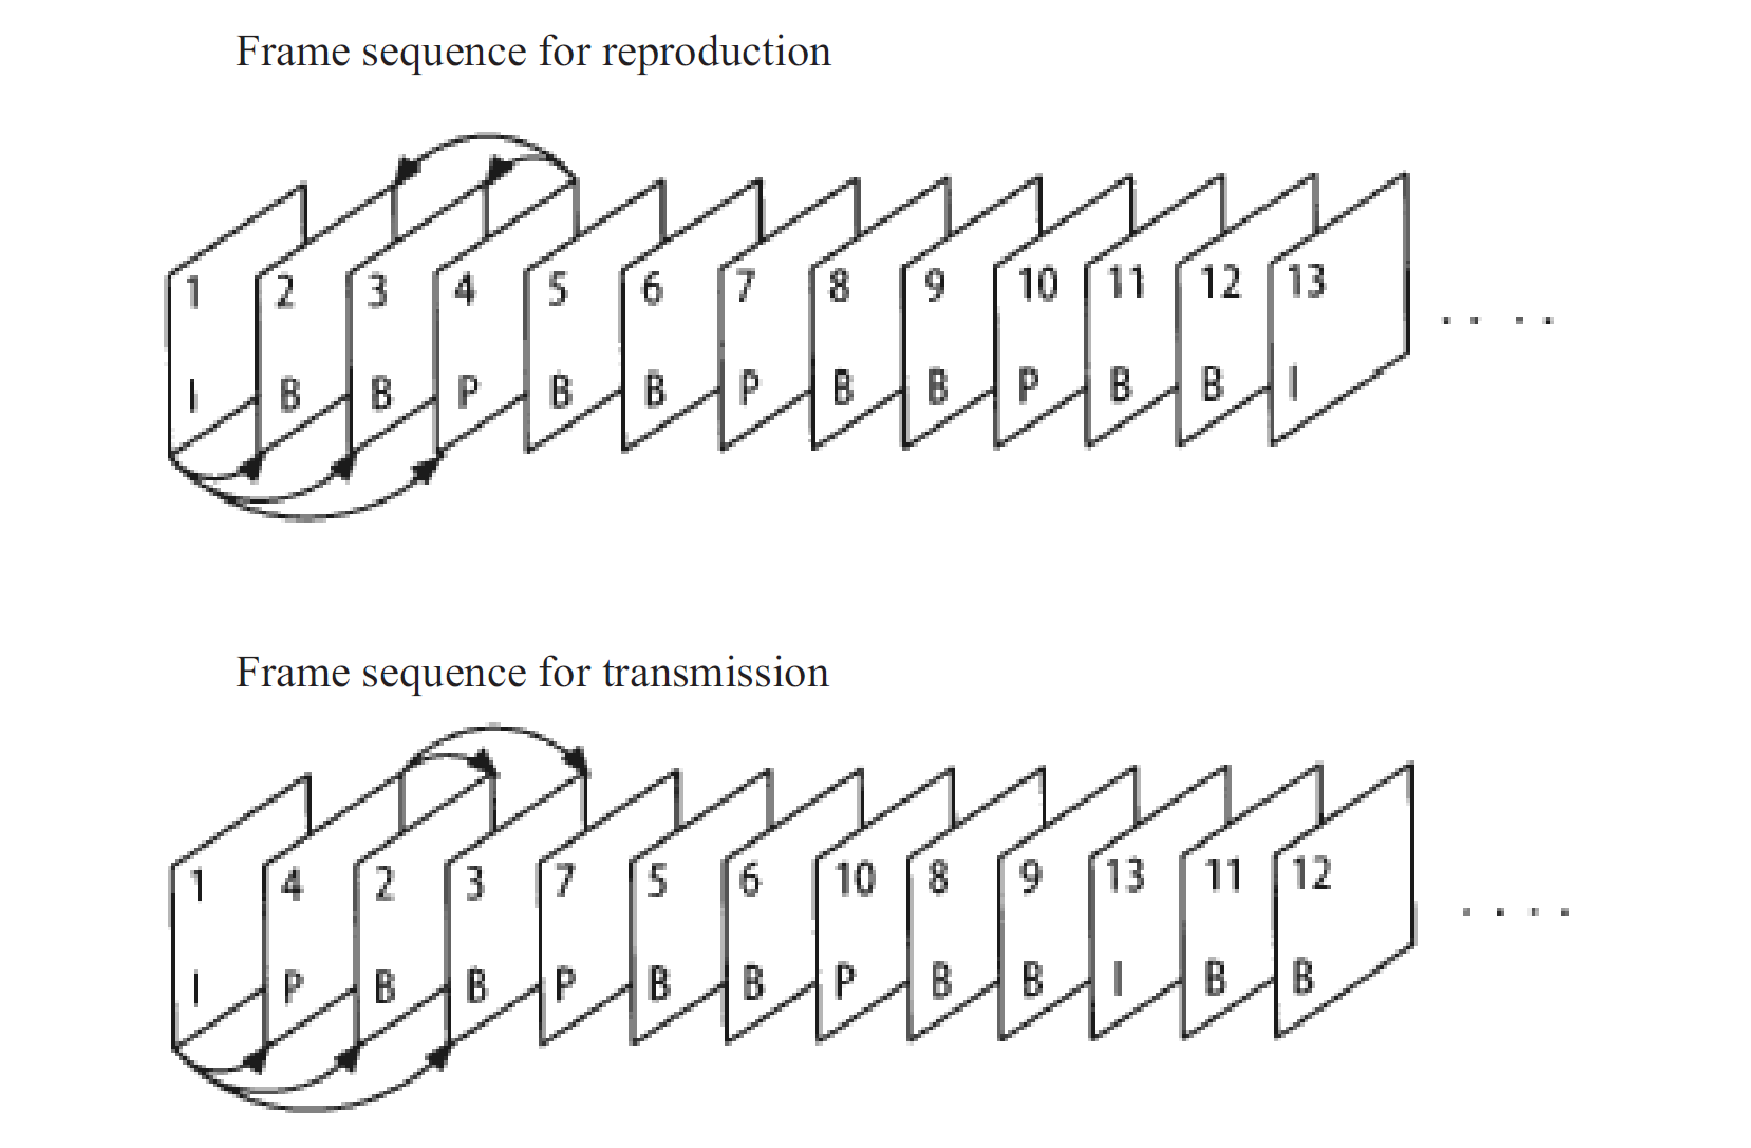
\includegraphics[width=0.4\textwidth]{../figures/frame_sequence_mpeg2.pdf}
  \caption{MPEG2 frame sequence \cite[p.98]{dsp_henkel}}
  \label{figure:mpeg2_frame_sequence}
\end{figure} 
\indent In a standardized Video Codec, only the bit steam and the decoding process and the choice of transforms are fixed by the standard in order to ensure compatibility across a broad range of devices and applications. The encoding process is not fixed and can be changed as long as the bitstream complies with the standard.      \cite{vsp_coursera} 

\subsection{VP9 coding standard}
VP9 is a modern Bandwidth-efficient video coding standard which was initially released by Google on the 17th of June 2013. It is a Hybrid Motion Compensated Video codec following it's general structure.  

\subsection{Screen Content Coding}
%define screene content

%the issue





\newpage
\section*{Bibliography}
\printbibliography

\end{document}
